\section{Hypothesis} \label{hypothesis} 

The proposed hypothesis suggests that both 'Clean Architecture' and 'Normalized Systems' lead
to modular software architectures with reduced combinatorial effects. Consequently, both
architectural approaches will lead to improved stability and evolvability of the
Information system.

Both architectural approaches formulate their modular structures independent of any
given programming technology \parencite[]{mannaert_normalized_2009,martin_clean_2018}.As
such, improvements in terms of stability and evolvability are equally applicable for the
C\# artifact used in this research, compared to case studies where Java SE has been used.
\parencites[]{oorts_building_2014, de_bruyn_enabling_2018}.

\begin{figure}[!ht]
    \centering
    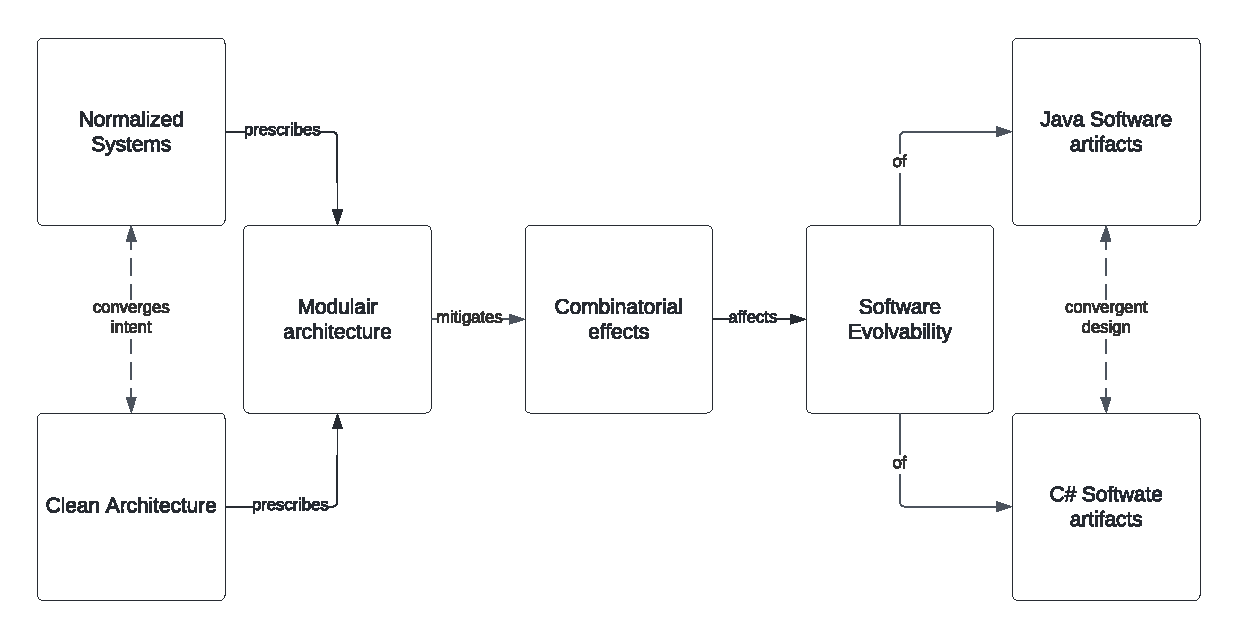
\includegraphics[width=0.9\textwidth]{Figures/hypothesis.pdf}
    \caption[The hypothesis]{The hypothesis}
    \label{fig_hypothesis}
\end{figure}